\section{Preliminary results}
\label{sec:preliminary_results}
As described in figure~\ref{fig:ov_tool}, the proposed framework for tract segmentation has two main steps: creating hypo candidate from whole brain tractogprahy base on supervised learning, and refining candidate using unsupervised learning. How to create tractography from the raw dMRI data can be found in our technical report~\cite{bao2012dmri}. The hypo generation step is inherited from the work in~\cite{olivetti2011supervised}, and our main investigation in this project focuses on the refinement step. In this part, we only present some preliminary results involved to the refinement step. First, the investigation of the dissimilarity approximation for tractography will be presented in section~\ref{subsec:result_dissimilarity}. The next section~\ref{subsec:resul_spagheti} describes Spaghetti, a streamline interaction visualization tool, which is the implementation of the framework in figure~\ref{fig:ov_tool}. The last section~\ref{subsec:result_ALS} shows a clinical application of the segmentation on finding the difference of CST~\footnote{Corticol Spinal Tracts: \url{http://dti-challenge.org/}} between healthy and ALS-diseased brains~\footnote{Amyotrophic Lateral Sclerosis: \url{http://www.alsa.org/}}.
%inspira ted from   Our method has these main steps: pre-processing the raw dMRI data to get the tractography in standard format~\cite{bao2012dmri}, presenting the tractography in a vector space using dissimilarity approximation tractography\cite{olivetti2012approximation}, and applying machine learning techniques -\textbf{supervised and fast clustering-unsupervised} to help segmentation the tractography. After that, the segmentation result is applied for ALS disease diagnosis.
%Forward the final result, up to present, we have some premilinary results. The first one is the approximation of dissimilarity for tractography, which is used as a method to represent tracts in a common space necessary for machine learning technique~\cite{olivetti2012approximation}. The second one is an interaction visualization tool be able to help medical practitioners to perform the tract segmentation task easily~\cite{garyfallidis2012software}. The last one focuses on the earlier diagnose ALS disease by finding the difference of Corticol Spinal Tracts between healthy and ALS-diseased brains.
%\subsection{dMRI pre-processing}
%\label{subsec:dMRI_pre-processing}
%Diffusion imaging is a method for measuring the displacement distribution of water molecules in vivo. From the displacement distribution, we can infer the fibre orientation or orientations in each imaging volume element (or voxel). More recently, several groups have proposed tractography methods and have reported success in following fiber tracts. However, there are still some problems with the dataset for doing these things. First, the resolution and quality of diffusion images in vivo was not adequate for this demanding application. Second, the macroscopic fibertract direction field is obtained from measured dMRI data that is discrete, coarsely sampled, and noisy. It is difficult to construct fluid streamlines accurately from discrete, noisy, velocity field data. A pre-processing stage which is capable of generating a continuous, smooth representation and highly standard of the measured dMRI data first has to be done in order to ensure the reliability and robustness of dMRI fiber tractography. The aim of this stage is to propose and describe a process to perform tractography from discrete measured diffusion tensor MRI data. 
%This process is running in Python language to find fiber tracts in the brain using the dataset of Cambridge university. For the better visualization, the tractography will be presented in FSL\footnote{FSL is a comprehensive library of analysis tools for FMRI, MRI and DTI brain imaging data~\url{http://www.fmrib.ox.ac.uk/fsl/}} and doctors can see and manipulate directly on it. 
%From the actual raw dMRI data we can create the tractrography as the following sequence. Frist, the raw data usually in DICOM (Digital Imaging and Communications in Medicine) format has to convert to NIfTI (Neuroimaging Informatics Technology Initiative) format by using NiBabel,~\footnote{\url{http://nipy.org/nibabel}} a pure python package, and easy to run on any system. Because DICOM data is quite complex leading to difficultly understanding, while NIfTI is simple, compact, versatile and includes important information like the orientation of the image, which is useful f	or scientific analysis of brain images.
%Second, the reconstruction step is active to extract information about orientation of fibres at every voxel. Based on this information, we can connect these directions to reconstruct complete tracks. This step is known as tracking~\cite{mori2002fiber}, which connect voxels in order to create tracks, or streamlines. The most popular algorithm for tracking is \emph{deterministic tractography}~\cite{mori2002fiber}. By using it, we can reconstruct white matter fiber tracts as a set of \emph{streamlines}, also known as \emph{tracks} (figure ~\ref{Fig:tracking}). A streamline is a mathematical approximation of thousands of neuronal axons expressing anatomical connectivity between different areas of the brain, see figure~\ref{fig:streamlines}.
%\begin{figure} 
%  \centering 
%  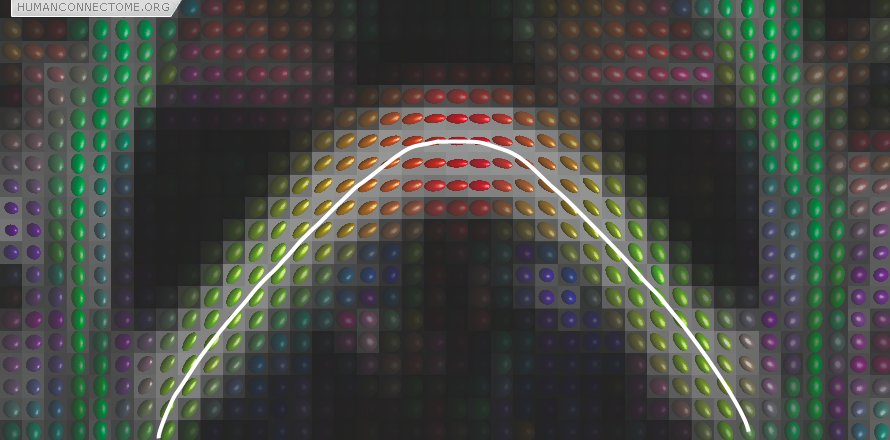
\includegraphics[width=4.5cm]{tensor_trajectory.jpg}
%  \caption{Tracking from tensor direction information}
%  \label{Fig:tracking}
%\end{figure}
%The last step is coregistration from native space to MNI (Montreal Neurological Institute)~\footnote{\url{http://www.mni.mcgill.ca/}} space. The reason is that all these tractographies were initially in native space or space of scanner. Because each measurement has it own coordinator, and this makes doctors or neuroscientists very difficult to compare, integrate or further study the tractography (see in figure ~\ref{Fig:sub1sub9coregister}). They are needed to be warped into the common space. In the other way, registration is the process of transforming from native space into the coordinate system~\cite{zvitia2010coregistration}. More detail about these steps can be found in ~\cite{bao2012dmri}.
%\begin{figure}
%  \centering
%  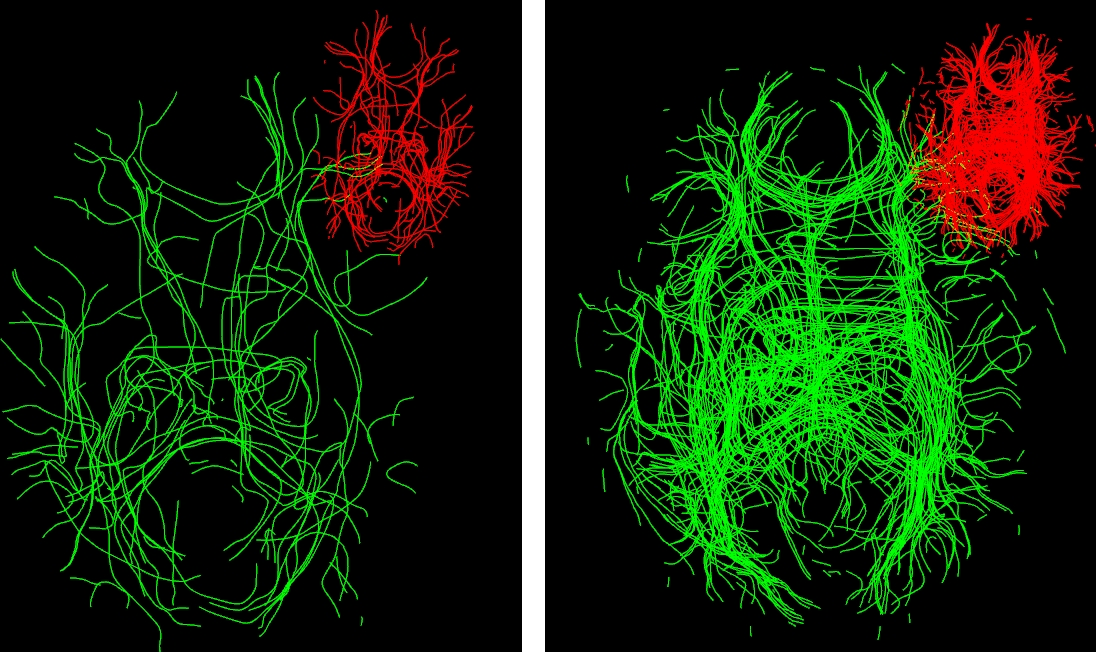
\includegraphics[width=4.5cm]{sub1_sub9_coregistering.jpg}
%  \caption{Tractography before(green) and after(red) the coregistration. Subject 1(left) and 9(right) of Cambrigde dataset}
%  \label{Fig:sub1sub9coregister}
%\end{figure}
\subsection{Tractography dissimilarity approximation}
\label{subsec:result_dissimilarity}
%Due to the lack of time, up to present, we only had experiment on dissimilarity approximation for tractography. 
In this section we describe the assessment of the degree of approximation of the dissimilarity representation across different prototype selection policies and different numbers of prototypes \cite{olivetti2012approximation}. The aim is to investigate the trade-off between accuracy and computational cost. The robustness of the method is checked first using simulated data, and then on the real tractography. But in the following, we only describe the experiment on real dMRI data. More detail about these experiments can be found in our recent publication~\cite{olivetti2012approximation} at PRNI-2012~\footnote{http://www.mlnl.cs.ucl.ac.uk/prni2012/} %The experiments are carried out on real tractographies reconstructed from dMRI recordings of the human brain.

We estimated the dissimilarity representation over real tractography data from dMRI recordings %of the MRI facility 
at the Cognition and Brain Sciences Unit, Cambridge, United Kingdom. The dataset consisted of $12$ healthy subjects; $101$ ($+1$, i.e. $b=0$) gradients; $b$-values from 0 to 4000; voxel size: $2.5 \times 2.5 \times 2.5 mm^3$. 
In order to get the tractography, 
% we computed the single tensor reconstruction (DTI) and created the streamlines using EuDX, 
we used the deterministic tracking algorithm~\cite{garyfallidis2012towards}.
% from the DiPy~\footnote{\url{http://www.dipy.org}}library. 
We obtained two tractographies using $10\times 10^3$ and $3\times10^6$ random seeds respectively. The first tractography consisted of approximately $10^3$ streamlines and the second one of $3\times 10^5$ streamlines. We used all three policies of choosing prototype: random, FFT and SFF. An example of a set of prototypes from $3\times10^5$ streamlines is shown in figure~\ref{fig:streamlines}. As the distance between streamlines we chose the most common one, i.e. the mean average minimum (MAM) distance from~\cite{zhang2008identifying} defined as $d_{mam}(s,s') = \frac{1}{2}(\delta(s,s') + \delta(s,s'))$ where
\begin{equation}
  \label{eq:mam_distance}
  \delta(s,s') = \frac{1}{|s|} \sum_{\mathbf{s}_{i} \in s}
    \min_{\mathbf{s'_j} \in s'} ||\mathbf{s}_i - \mathbf{s'}_j||_2.
\end{equation}
As shown in figure~\ref{fig:correlation_1K}(left), in the case of the $10^3$-streamline tractography, both FFT and SFF ($c = 3$) had significantly higher correlation than the random sampling for all numbers of prototypes considered. We confirmed that the SFF selection policy is an accurate approximation of the FFT policy for tractographies. Moreover we noted that after $15-20$ prototypes the correlation reached approximately $0.95$ on average ($60$ repetitions) and then slightly decreased indicating that a little number of prototypes was sufficient to reach a very accurate dissimilarity representation.
\begin{figure}
  \centering
  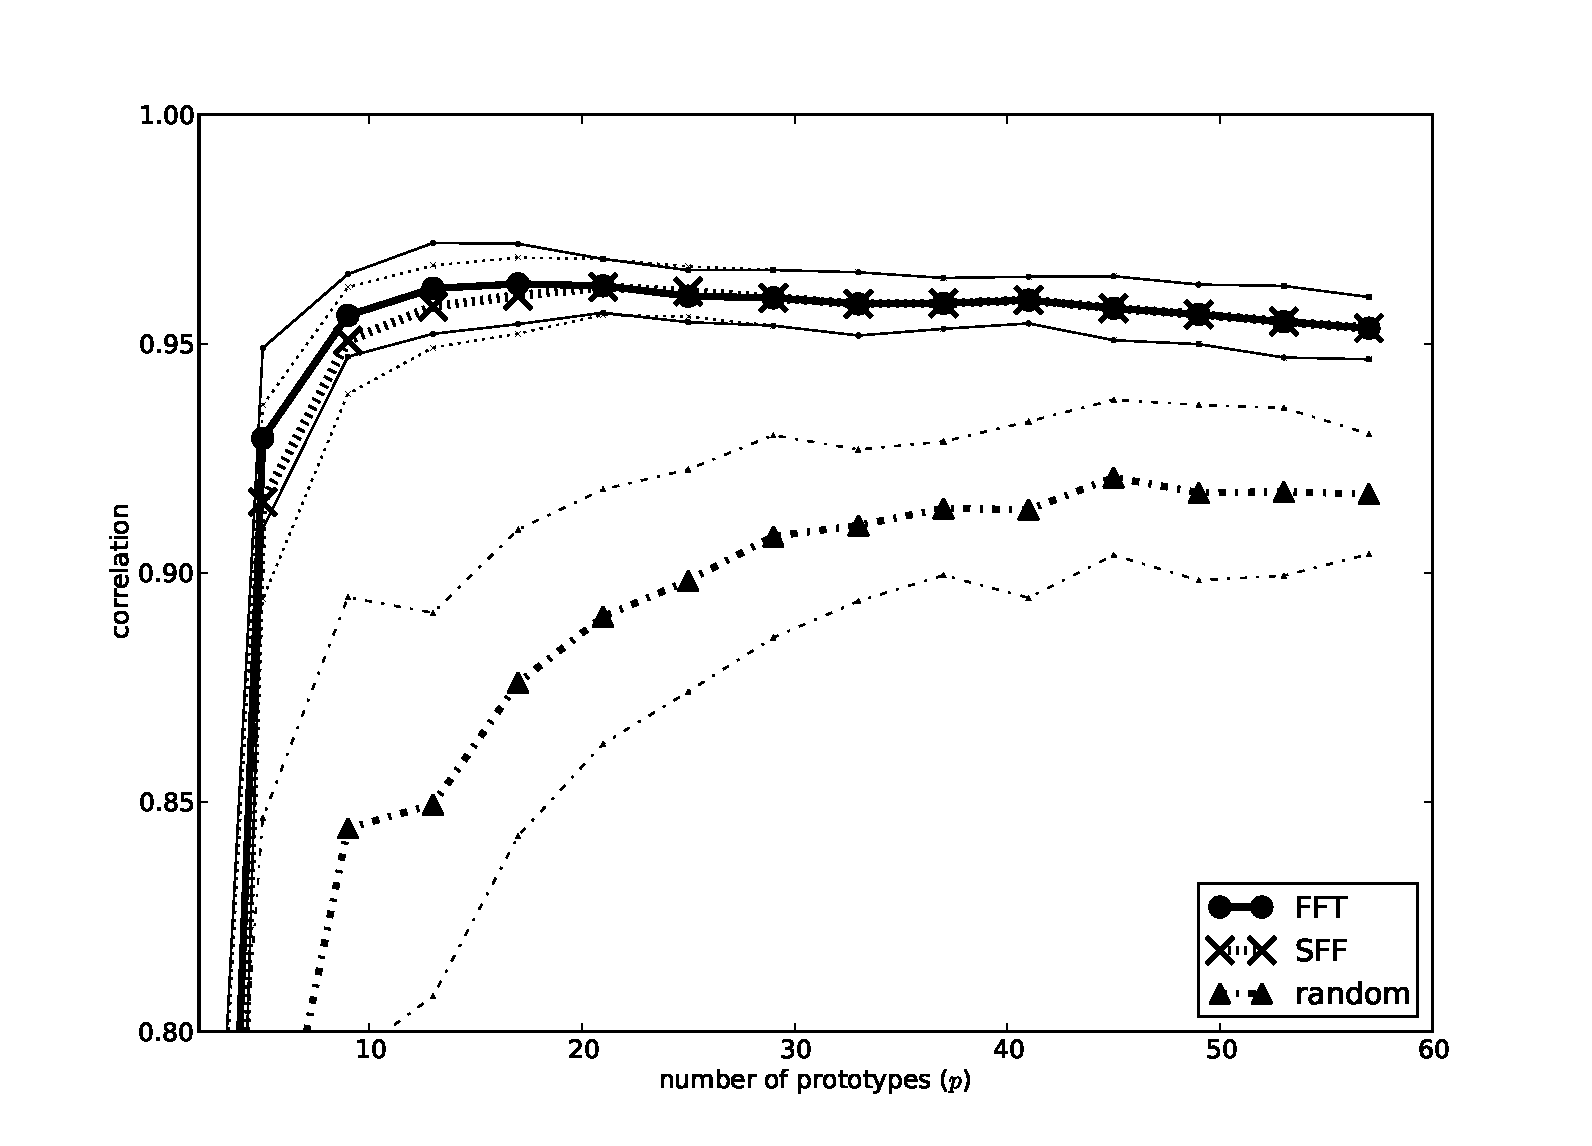
\includegraphics[width=4.5cm,height=3.85cm]{120323_file_120322_15h_subj1_60_4pro_c10_500tracks_allpairs_alltracksforpro_score_gen_9line_new.pdf}
  \includegraphics[width=4.1cm,height=3.85cm]%[bb=5 -5 80 80][bb=5 5 40 40]%
  {120323_file_120322_15h_subj1_100_5pro_c10_1000tracks_allpairs_alltracksforpro_score_gen_9lines.pdf}
  \caption{The correlation between of $d$ and $\Delta_{\Pi}^d$ over a
   tractography for different prototype selection policies: $\mathbf{10^3}$ streamlines (left) and $\mathbf{3\times 10^5}$ streamlines (right).}
  \label{fig:correlation_1K}
\end{figure}
%\begin{figure}
%  \centering
%  \includegraphics[width=6.5cm,height=3.85cm]%{120323_file_120322_15h_subj1_100_5pro_c10_1000tracks_allpairs_alltracksforpro_score_gen_9lines.pdf}
%  \caption{The correlation between of $d$ and $\Delta_{\Pi}^d$ for a
%    full tractography of $\mathbf{300K}$ streamlines for the random and SFF
%    prototype selection policies.}
%  \label{fig:correlation_300K}
%\end{figure}
Figure~\ref{fig:correlation_1K}(right) shows the correlation between SFF and the random policy when the tractography has $3\times 10^5$ streamlines, i.e. the standard size of a tractography from current dMRI recording techniques. In this case, FFT was impractical to be computed because it required approximately $15$ minutes on a standard desktop computer for a single repetition when $p=60$. The cost of computing SFF was instead the same of the case of $10^3$ streamlines, as its computational cost depended only on the number of prototypes. It took $\approx 2$ seconds on standard desktop computer when $p=60$ to compute one repetition. We observed that for $3\times 10^5$ streamlines, SFF significantly outperformed the random policy and reached the highest correlation of $0.96$ on average ($60$ repetitions) for $15-25$ prototypes. Note that the figures presented in this section refers to data from subject $1$ of the dMRI dataset. We conducted the same experiments on other subjects obtaining equivalent results. 

All of the results from both simulated data and real tractography data reached correlation $\geq 0.95$, showing a strong evident that dissimilarity approximation works well for preserving the relative distances. We advocate that the dissimilarity representation can produce compact feature spaces for the tractography. Moreover we strongly suggest the use of the SFF policy to obtain an efficient and effective selection of the prototypes.
\subsection{Spaghetti: an interaction visualization tool for tract segmentation}
\label{subsec:resul_spagheti}
In this part, we present a streamline interaction visualization tool, called Spaghetti, which is the implementation of the framework in figure~\ref{fig:ov_tool}. But until now, we have not integrated the hypo generation step in this tool yet. It is supposed to use the whole tractography $\mathbb{T}$ instead of a set of candidates $\mathcal{T}$.
%The main purpose of this scientific tool is to support medical practitioners to do the tract segmentation task more easy.
% Be honestly, interacting with tractography is a difficult procedure for various reasons: (a) tractographies are usually represented by hundreds of thousands of intertwined streamlines see~\ref{fig:tractography}; (b) data sets are often cluttered with noisy tracks, i.e. tracks which have no relevance in anatomy; (c) the size of the entire tractography is often too large to load in the memory of the graphics card; (d) navigating specific regions of a tractography in $3D$ space is cumbersome because of the unique shape characteristics of the streamlines. We build up an interactive tool that solves these problem.
%of interacting with tractographies by creating real-time simplifications in terms of the underlying bundle structures. 
The process that we propose works recursively: starting from a small number of clusters of streamlines the user decides which clusters to explore. Exploring a cluster means that the application re-clusters its content at a finer grained level or provides the content (means streamlines) of that cluster. In another words, the users change the level of abstraction and we provide cluster representatives of new clusters according to that level. % they want to look at the tractography, 

As the distance between streamlines, beside the MAM (equation~\ref{eq:mam_distance}, we also use the MDF (minimum average direct flip)
%$d_{mdf}(s,s') = min(\delta_{direct}(s,s'),\delta_{flipped}(s,s'))$
\begin{equation}
\label{eq:mdf_distance}
	d_{mdf}(s,s') = min(\delta_{direct}(s,s'),\delta_{flipped}(s,s'))
\end{equation}
with $\delta_{direct}(s,s') = \frac{1}{k} \sum_{i=1}^{k} 
	||\mathbf{x}_{i} - \mathbf{x'}_i||_2.$
and $\delta_{flipped}(s,s') = \frac{1}{k} \sum_{i=1}^{k} 
	||\mathbf{x}_{i} - \mathbf{x'}_{k-i}||_2.$
%\begin{equation}
%\label{eq:dirrect}
%	d_{direct}(s,s') = \frac{1}{k} \sum_{i=1}^{k} 
%	||\mathbf{x}_{i} - \mathbf{x'}_i||_2.
%\end{equation}
%\begin{equation}
%\label{eq:dirrect}
%	d_{flipped}(s,s') = \frac{1}{k} \sum_{i=1}^{k} 
%	||\mathbf{x}_{i} - \mathbf{x'}_{k-i}||_2.
%\end{equation}
where $k$ is the number of points $\mathbf{x}_{i}$ on the two tracks $s$ and $s'$.
%\begin{equation}
%\label{eq:mam}
%	MAM_{mean}(s,s') = \frac{1}{2}(d_{mean}(s,s') + d_{mean}(s',s))
%\end{equation}
%\begin{equation}
%\label{eq:mean}
%	d_{mean}(s,s') = \frac{1}{k} \sum_{i=1}^{k}	d(\mathbf{x}_{i},s')
%\end{equation}
%\begin{equation}
%\label{eq:min}
%	d(\mathbf{x},s) = min_{j=1,\ldots,k}||\mathbf{x} - \mathbf{x'}_{j}||_2
%\end{equation}
In this software, currently we use the fast clustering algorithm proposed in~\cite{garyfallidis2012quickbundles}, called QuickBundle(QB). The reason is that QB is very simple, easy to implement and very fast. However, every time user change the level of abstraction, we need to re-run QB to get the new clusters. It is one of the drawbacks of the current version of Spaghetti.

The application starts visualizing the brain as a set of a few cluster representative.
%, i.e. the cluster representatives.
Each representative track acts as the access point to the streamlines within that cluster and allows the user to address this portion of the tractography as a single unit, which we call "bundle of interest" (BOI). After visually inspecting the simplified tractography the user interactively selects one or more representative tracks and explores them.
%When one or more representative tracks are selected the user can see the content of the related clusters. 
In order to explore the detailed %structure of content 
of the selection, the user may ask to re-cluster the selected BOIs, and possibly further refine the initial selection.
% into smaller clusters in order to address and possibly further refine the initial selection. 
%This procedure can repeat until user satisfies with the the local structures result.
After selecting one or more of the small clusters through their representatives the user can repeat the visual inspection step, and the re-clustering step as required in order to unveil the local structures.
\begin{figure}
	\centering
	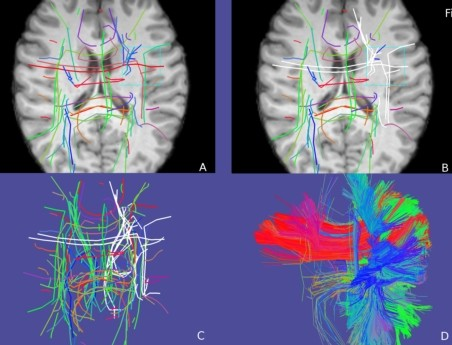
\includegraphics[height=3.85cm]{spaghetti1.jpg} %width=7.5cm
	\caption{Streamline interaction with Spaghetti: the initial representatives (A); some selected clusters in white color (B); only representatives without slices (C); exploring representatives by hundred of streamlines (D)}
  \label{fig:spaghetti}
\end{figure}
Beside the capability of interacting with streamlines, in this tool we also provide function of visualizing slices of structural volumes (see figure~\ref{fig:spaghetti}). The volume is aligned in the same space (e.g standard space) of the tractography.
% We also provide functions to move/hide these slicers . 
This enables medical practitioners and researchers to meaningfully navigate the entire space of the tractography related to anatomy. The detail of this tool can be found in our publication~\cite{garyfallidis2012software}  at OHBM-2012\footnote{Organization for Human Brain Mapping 2012~\url{http://www.humanbrainmapping.org/OHBM2012/}}
 %These representative tracks are provided by a very fast tractography clustering algorithm. %called QuickBundles~\cite{garyfallidis2012towards} which can cluster thousands of tracks in milliseconds. 
%~\cite{garyfallidis2012quickbundles}
%\subsection{Clinical diagnosis applications}
%Some text here
%\textbf{Diagnosis ALS disease}
%Some text here
%\textbf{Other disease here}
%Some text here
\subsection{Clinical diagnosis application: the difference of Corticol Spinal Tracts between a healthy and an ALS-diseased brain}
\label{subsec:result_ALS}
In this part, we try to demonstrate the usefulness of tract segmentation in clinical study. 
%Traditionally, diagnostic decision making has involved using evidence provided by patient's data coupled with physician's priori experience. Up to now, it is still very much an art for many physicians due to a lack of quantitative tools and measurements. 
The aims of this work are to: first, finding the differences of the Corticol Spinal Tracts (CST) between a healthy brain and an ALS (Amyotrophic Lateral Sclerosis) diseased brain based on tract quantification; and second present a general framework for clinical diagnosing based on the differences between two folders of interesting tracks.
%1) describe a process to perform tractography from discrete measured diffusion tensor MRI data of ALS-2012 dataset; 
%1) present a general framework for finding the differences between two folders of tracks based on tract quantification; and 2) demonstrate this process in finding the differences of the Corticol Spinal Tracts (CST) between a healthy brain and a patient.
%\begin{figure}
%  \centering
 % 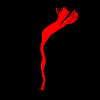
\includegraphics[bb=0 0 140 150]{201CTS1Mleft_1.png}
 % 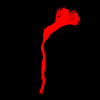
\includegraphics[bb=0 0 140 150]{201CTS3Mleft_1.png}%[bb=0 0 200 300]
 % \caption{The left CTS segmentation of control 201 in the dataset ALS\underline{ }Nivedita. The left image is the segmentation from the 1M tractography and has $154$ tracts. While the right is one from 3M tractography and the number of tracts is $487$.}
 % \label{fig:CTS_201_left}
%\end{figure}
\begin{figure}
  \centering
  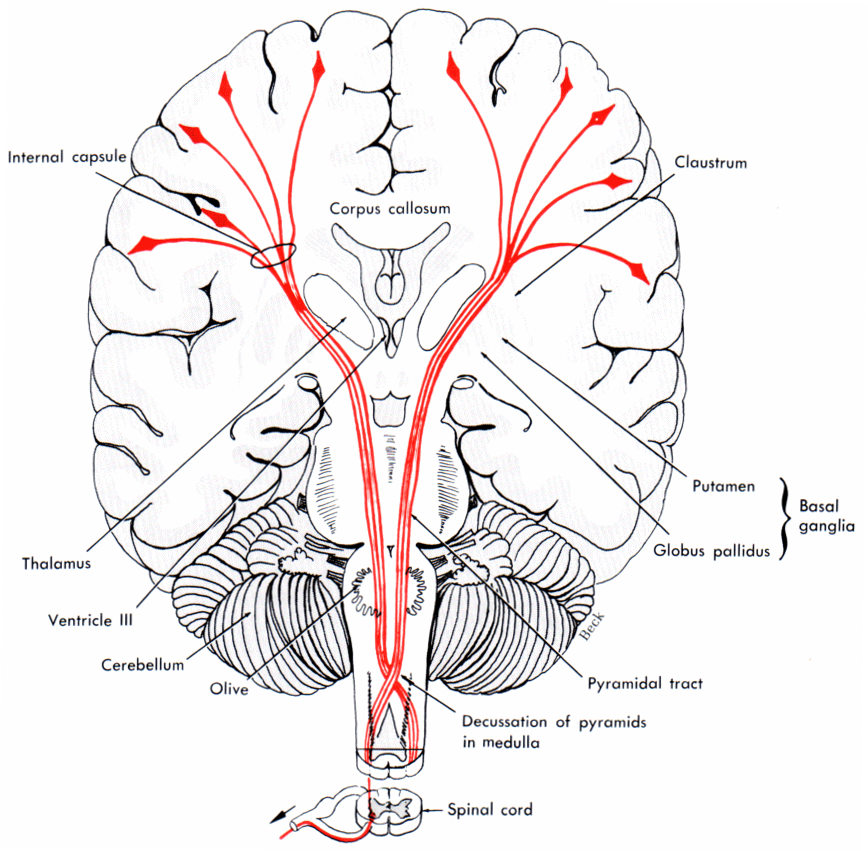
\includegraphics[width=4.2cm,height = 3.85cm]{CST.png}
  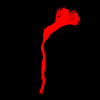
\includegraphics[bb=5 -5 80 80]{201CTS3Mleft_1.png}
  \caption{Left - the Cortico Spinal Tracts in general. Right - the left CST segmentation of the control 201 in the dataset ALS}%\underline{}Nivedita}%, from 3M tractography and the number of tracts is $487$}
  \label{fig:CST}
\end{figure}
%ALS, also known as motor neurone disease or Lou Gehrigs disease, is a fatal, progressive neuromuscular disease that attacks the motor neurons controlling voluntary movement. The result is wasting and atrophy of muscles, leading to difficulties in speaking or swallowing, stumbling, permanent fatigue and cramping, amongst other symptoms. 
\\\textbf{\textit{ALS}}, also known as motor neurone disease or Lou Gehrigs disease, is a progressive neurodegenerative disease that affects nerve cells in the brain and in the spinal cord. 
%Motor neurons reach from the brain to the spinal cord and from the spinal cord to the muscles throughout the body. 
As motor neurons degenerate, they can no longer send impulses to the muscle fibers that normally result in muscle movement. The result is wasting and atrophy of muscles, leading to difficulties in speaking, swallowing, stumbling, etc. %permanent fatigue and cramping, amongst other symptoms. Due to that fact that 
Because ALS disease involves to the nerve cells in \textit{\textbf{CST}}, in this part, we only focus on this CST tract.
%for diagnosing ALS we need to know the difference of CST between a healthy and an ALS-diseased brain. 
Usually, CST starts from the cerebral cortex, and terminates in the spinal cord. Note that fibers after crossing over from one side to the other
%, in the medulla, 
continue downward in the lateral corticospinal tract on the opposite side and go to muscles (see figure~\ref{fig:CST}-left). %Each crossed corticospinal tract, therefore, conducts motor impulses from one side of the brain on interneurons or anterior horn motoneurons on the opposite site of the cord. 
That is the reason why impulses from one side of the cerebrum cause movements of the opposite side of the body.

CST segmentation was done by doctors using Spaghetti tool on the ALS dataset, recorded with a $3T$ scanner at Utah Brain Institute. This dataset consisted of $12$ healthy controls and $12$ subjects; $64$ ($+1$, i.e. $b=0$) gradients; $b$-values $1000$; voxel size: $1. \times 1. \times 1. mm^3$. For creating tractography, we used the same algorithm in section~\ref{subsec:result_dissimilarity}, with $3\times 10^5$ random seeds. An example of CST segmentation from ALS dataset is in figure~\ref{fig:CST} (left). As the result, we had $48$ segmentations ($24$ of patients including $12$ left CST and $12$ right CST; and similar for controls).

From the prior knowledge of neuroscientists and doctors, there is an evidence about the reducing of the number of fibers in CST of ALS patients compared with control people. It is also the same situation with the volume of CST. Beside,
% the number of fibers and the volume, 
fractional anisotropy (FA) and mean diffusion (MD) also play an important role for recognizing the ALS disease. Following are some quantitative features which may effectively affect on ALS patients: \textit{fiber count} - the number of streamlines belonging to CST; \textit{fiber length} in $mm$ (min, max, mean length); \textit{fiber volume} - number of voxels occupied by all streamlines or the bounding geometry cylinder of CST; \textit{fiber density} - ratio between fiber count and voxel number; \textit{fragmentation} - %can be quantified by the 
ratio between fiber count and the volume; \textit{fractional anisotropy (FA)} - defined as mean value of the standard deviation in the three eigenvalues and in the range $0$ to $1$
	\begin{equation}
   FA=\frac{1}{\sqrt{2}}\frac{\sqrt{(\lambda_{1}-\lambda_{2})^{2}+(\lambda_{2}-\lambda_{3})^{2}+(\lambda_{3}-\lambda_{1})^{2}}}{\sqrt{\lambda_{1}^{2}+\lambda_{2}^{2}+\lambda_{3}^{2}}}
   \label{eq:FA}	
\end{equation} 
and \textit{mean diffusion (MD)} - the average diffusion rate in all directions% $MD=\frac{1}{3}(\lambda_{1}+\lambda_{2}+\lambda_{3})$ 
	\begin{equation}
   MD=\frac{trace(DT)}{3}=\frac{\lambda_{1}+\lambda_{2}+\lambda_{3}}{3}
%	   MD=\frac{\lambda_{1}+\lambda_{2}+\lambda_{3}}{3}
   \label{eq:MD}	
\end{equation}
%
%\begin{itemize}
%	\item fiber count: the number of streamlines belonging to CST
%	\item fiber min/max/mean length: length in $mm$% for all streamlines belonging to CST
%	\item fiber volume: number of voxels occupied by all streamlines or the bounding geometry cylinder of CST
%	\item fiber density: ratio between fiber count and voxel number
%	\item FA: defined as mean value of the standard deviation in the three eigenvalues and in the range $0$ to $1$
%	\begin{equation}
 %  FA=\frac{1}{\sqrt{2}}\frac{\sqrt{(\lambda_{1}-\lambda_{2})^{2}+(\lambda_{2}-\lambda_{3})^{2}+(\lambda_{3}-\lambda_{1})^{2}}}{\sqrt{\lambda_{1}^{2}+\lambda_{2}^{2}+\lambda_{3}^{2}}}
%   \label{Equ:FA}	
%\end{equation}
%	\item MD: the average diffusion rate in all directions 
%	\begin{equation}
%   MD=\frac{trace(DT)}{3}=\frac{\lambda_{1}+\lambda_{2}+\lambda_{3}}{3}
%	   MD=\frac{\lambda_{1}+\lambda_{2}+\lambda_{3}}{3}
%   \label{Equ:MD}	
%\end{equation}
%	\item fragmentation: %can be quantified by the 
%	ratio between fiber count and the volume
%\end{itemize}
where ($\lambda_{1}, \lambda_{2}, \lambda_{3}$) is eigenvalues of diffusion at a given voxel.
\\After calculating the value of these features, we did a $t-test$ on each set of left and right. It showed that, in the right CST, fiber number significantly decreased $(p = 0.00042)$ in ALS patients ($mean_{fiber-number} = 294$) compared with controls ($mean_{fiber-number} = 640$). In contrast, patients had the fiber min length slightly higher then controls ($p=0.07$, patients: $mean_{min-length}= 74.25$ and controls: {$mean_{min-length} = 53.9$). Moreover, the volumn of the left CST dramatically diminished ($p=0.0034$) between patients ($mean_{volumn}=6038$) and healthy peoples ($mean_{volumn}=4230$). These are just some preliminary results and it needs more investigation to confirm the difference between healthy and ALS-diseased brain. But it also shows an strong evidence that the tract segmenation has a bright capability for applying in clinical diagnose application.
%The CST converges in the subcortical white matter (corona radiata) and courses through the posterior limb of the internal capsule, the cerebral peduncle of the midbrain, the ventral pons (basis pontis), the ventral surface of the medulla, decussate in the lower medulla (pyramidal decussation). The figure~\ref{fig:CST} shows a visualization of CST. In this figure, axons that compose pyramidal tracts come from neuron cell bodies in the cerebral cortex. After they descend through the internal capsule of the cerebrum and the white matter of the brainstem, about three fourths of the fibers decussate cross over from one side to the other, in the medulla. After that, the fibers continue downward in the lateral corticospinal tract on the opposite side of the cord. Each crossed corticospinal tract, therefore, conducts motor impulses from one side of the brain on interneurons or anterior horn motoneurons on the opposite site of the cord. That is the reason why impulses from one side of the cerebrum cause movements of the opposite side of the body.
